\documentclass[12pt,a4paper]{article}
\usepackage{a4wide}

\usepackage{JohnMath}

\usepackage[svgnames]{xcolor}

% CODE LISTINGS
\usepackage{listings}
\lstset{
  language=C,
  columns=[l]fullflexible,
  mathescape=true,
  basicstyle=\ttfamily\color{Purple},
  showstringspaces=false,
  commentstyle=\color{DarkGreen}, 
  numbers=none, 
  escapechar=£,
  escapebegin=\normalsize\rmfamily\color{Black}
}


% SPECIFICATIONS
\newcommand{\ml}[2][t]{\mbox{\mdseries\begin{tabular}[#1]{@{}L@{}}#2\end{tabular}}}
\newcommand{\ass}[1]{\ensuremath{{\color{blue}\left\{\ml[c]{#1}\right\}}}}
\newcommand{\seqspec}[3]{\ass{#1}\,{\mbox{{\tt #2}}}\,\ass{#3}}
\newcommand{\Seqspec}[3]{\multicolumn{2}{l}{$\ass{#1}$ {#2} $\ass{#3}$}}
\newcommand{\comm}[1]{\vspace{-2pt}%
    \begin{list}{/$*$}{%
        \topsep=5pt%
        \leftmargin=3cm%
      }\item #1 \hfill$*$/\end{list}%
}

\newcommand{\checkthis}{$^{\rm [check\ this]}$}
\renewcommand{\floor}[2][]{\left\lfloor{#2}\right\rfloor_{#1}}
\renewcommand{\ceil}[2][]{\left\lceil{#2}\right\rceil_{#1}}
\newcommand{\floorpow}[1]{\llfloor{#1}\rrfloor}
\newcommand{\fracpow}[1]{\{\hspace{-3pt}\{{#1}\}\hspace{-3pt}\}}

% STATUS FLAGS
\newcommand{\setC}{\raisebox{1.5pt}{$\blacktriangledown$}}
\newcommand{\unsetC}{\raisebox{1.5pt}{$\triangledown$}}
\newcommand{\setP}{{\blacktriangle}}
\newcommand{\unsetP}{{\triangle}}

% BIT OPERATIONS
\newcommand{\AND}{\mathbin{\texttt{\&}}}
\newcommand{\OR}{\mathbin{\texttt{|}}}
\newcommand{\NOT}{\mathbin{\textasciitilde}}
\newcommand{\SHIFTRIGHT}{\mathbin{\texttt{>}\hspace{-1pt}\texttt{>}}}
\newcommand{\SHIFTLEFT}{\mathbin{\texttt{<}\hspace{-1pt}\texttt{<}}}

\newcommand{\doublestar}{{*\hspace{-3pt}*}}

\title{Verifying overlapping datastructures}
\author{John Wickerson}
\date{}

\begin{document}

\maketitle


Figure~\ref{fig:contrived} shows a simple overlapping datastructure. It is overlapping in the sense that we have two edge sets imposed on the same set of nodes. Each node is a struct comprising a {\tt val}, a brown `{\tt next}' pointer, and a green `{\tt fd}' pointer. The brown {\tt next} pointers form a chain, starting at {\tt start}, of all the nodes in which {\tt val} is non-decreasing. The {\tt mod} array identifies four equivalence classes, obtained by identifying {\tt val} fields modulo 4. The green {\tt fd} pointers form a circular singly-linked list that encompass all of the nodes in the same equivalence class, in any order. We use casting tricks to treat the {\tt start} pointer as a sentinel node in the linked list, and, likewise, each element of {\tt mod} as a sentinel node in its equivalence class.

\begin{figure}[tbp]
\centering
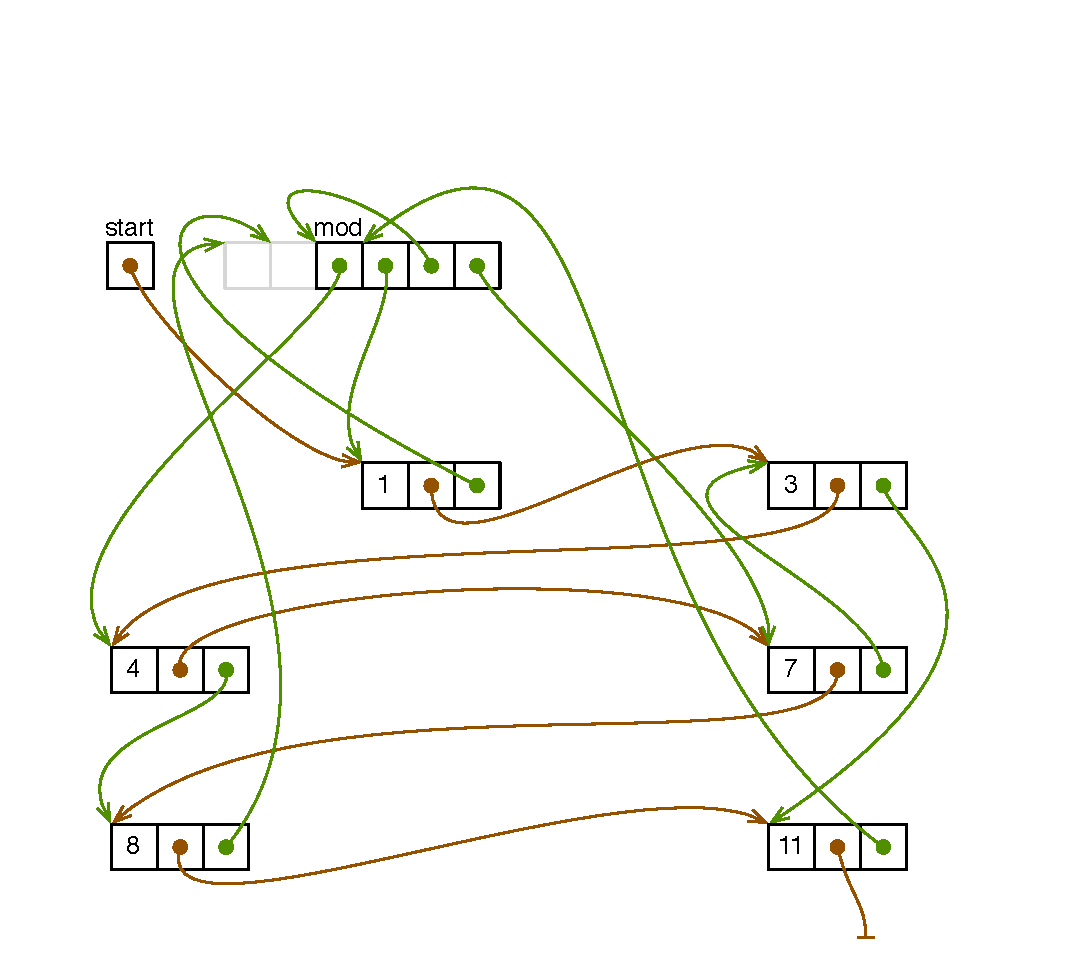
\includegraphics[width=75mm]{contrived.pdf}
\caption{An overlapping datastructure. We have no ownership of grey-outlined cells.}
\label{fig:contrived}
\end{figure}

We now consider several attempts to reason about this datastructure.

\section{Inductive predicate for the whole datastructure}

We might first try to find a predicate $p$ to describe the structure as a whole, in the same vein as the $list$ or $tree$ predicates in separation logic. Note that a naïve attempt of the form 
\[
p(x) ⇔ \ldots * x.{\tt next}↦y * x.{\tt fd}↦z * p(y) * p(z)
\]
fails because, unlike for lists or trees, $y$ and $z$ need not be distinct. So the predicate might look more like this:
\[
p_{m,n}(x) ⇔ \begin{array}[t]{l}(x.{\tt val}↦v ∧ v≥m ∧ v \text{ mod } 4 = n) {}\\{} * x.{\tt next}↦y * x.{\tt fd}↦z * \left\{\begin{array}{ll} p_{v,n}(y) & \text{if $y=z$} \\ p_{v,?}(y) * p_{?,n}(z) & \text{if $y≠z$}\end{array}\right. \end{array}
\]
But what to put for the two ?s is not clear at all. If node $x$ is in the $i^{\rm th}$ equivalence class, and its {\tt next} pointer points to node $y$, we do not know anything about $y$'s class -- it could be $i$ or any other. Yet not to specify $y$'s class at all would be to make $p$ too weak to capture the intended specification of the datastructure. The problem can be stated by saying that the datastructure is not built inductively.

\section{Fractional permissions}

Perhaps we are decomposing the structure in the wrong way. Perhaps we should not break the structure down into its individual nodes just yet: instead, let us first separate the two overlapping structures. I'm imagining an overall description of the state of this form:
\[
state ≝ \begin{array}[t]{@{}l} {\tt start}↦x * {\tt mod}↦c_0,c_1,c_2,c_3 {}\\{} * list(x) * class_0(c_0) * class_1(c_1) * class_2(c_2) * class_3(c_3) \end{array}
\]
How might we split nodes? The {\tt next} field clearly belongs to the $list$, and the {\tt fd} field belongs to the $class$. But the {\tt val} field needs to be available to both: the $list$ predicate needs to specify that {\tt val} doesn't decrease, while the $class$ predicate needs to know {\tt val} module 4. Let us use fractional permissions: let each predicate reason about half the {\tt val} field. The $list$ and $class$ predicates can then be implemented as follows:
\[
\begin{array}{rcl}
list_n(x) &⇔& x\dot= 0 ∨ ∃v,x'. x\dot{≠}0 * (x.{\tt val}\pto[.5] v ∧ v≥n) * x.{\tt next}↦x' * list_v(x') \\
list(x) &≝& list_0(x) \\
class_i(c) &⇔& c\dot={\tt mod}{+}i{-}2 ∨ ∃v,c'. c\dot{≠}{\tt mod}{+}i{-}2 * (c.{\tt val}\pto[.5]v ∧ v\text{ mod }4 = i) * c.{\tt fd}↦c' * class_i(c') \\
\end{array}
\]

The two overlapping structures are visualised in Fig.~\ref{fig:twoparts}. It is clear that when the two structures are superimposed, we attain the full picture of Fig.~\ref{fig:contrived}.

\begin{figure}[tbp]
\centering
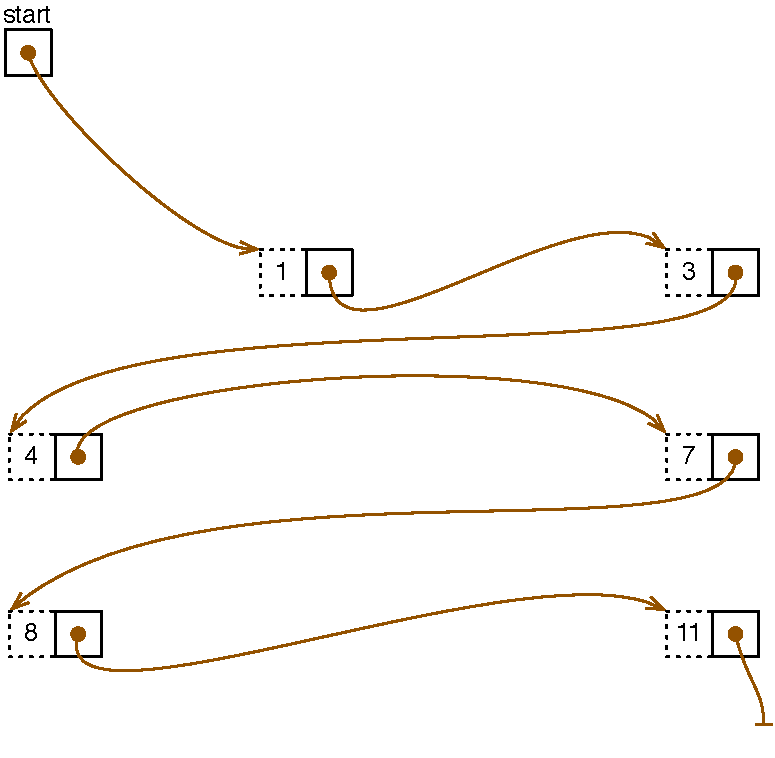
\includegraphics[width=50mm]{inclist.pdf} \hfil
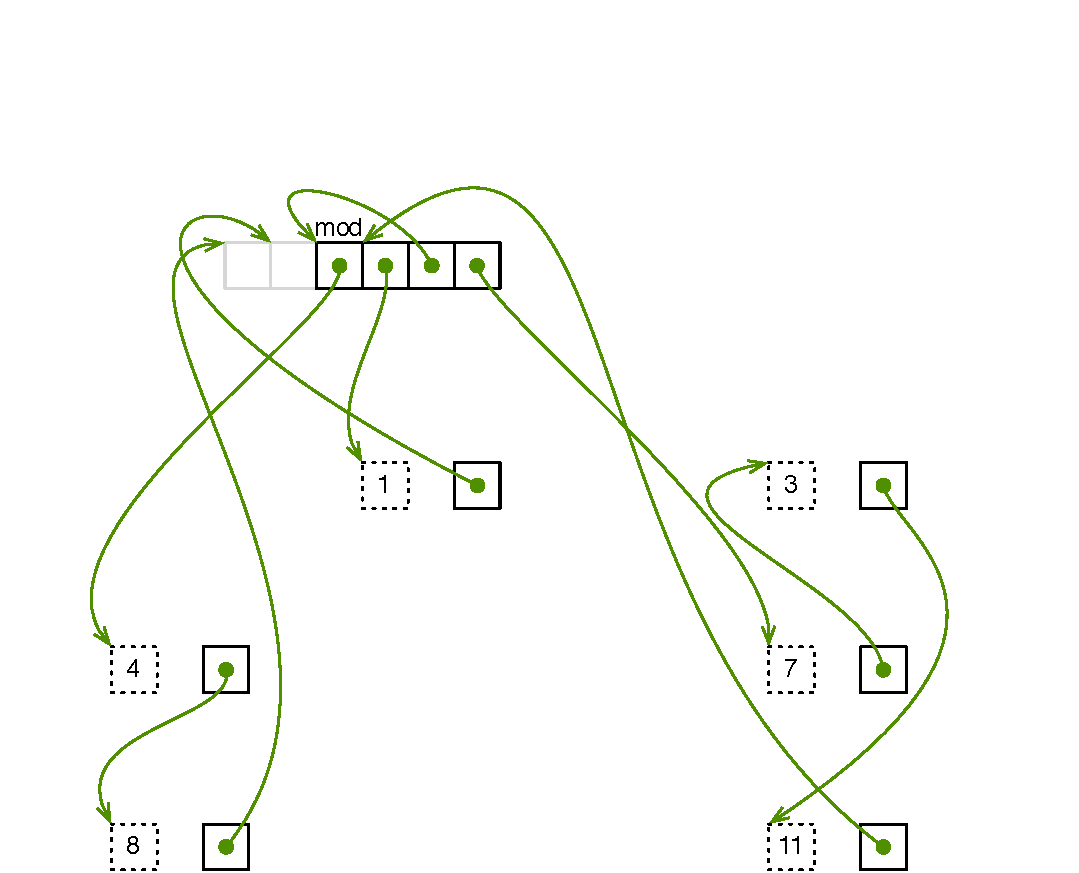
\includegraphics[width=75mm]{classes.pdf}
\caption{The $list$ and $class_i$ parts of the datastructure. We have half ownership of dotted-outlined cells.}
\label{fig:twoparts}
\end{figure}

Unfortunately, there is not enough consistency between the two descriptions. The $state$ predicate to specify that the four equivalence classes should contain all of the nodes that are in the increasing list, and that the increasing list should contain all of the nodes that are in one of the four classes. This means that it describes undesirable states such as that depicted in Fig.~\ref{fig:undesirablestate}.

\begin{figure}[tbp]
\centering
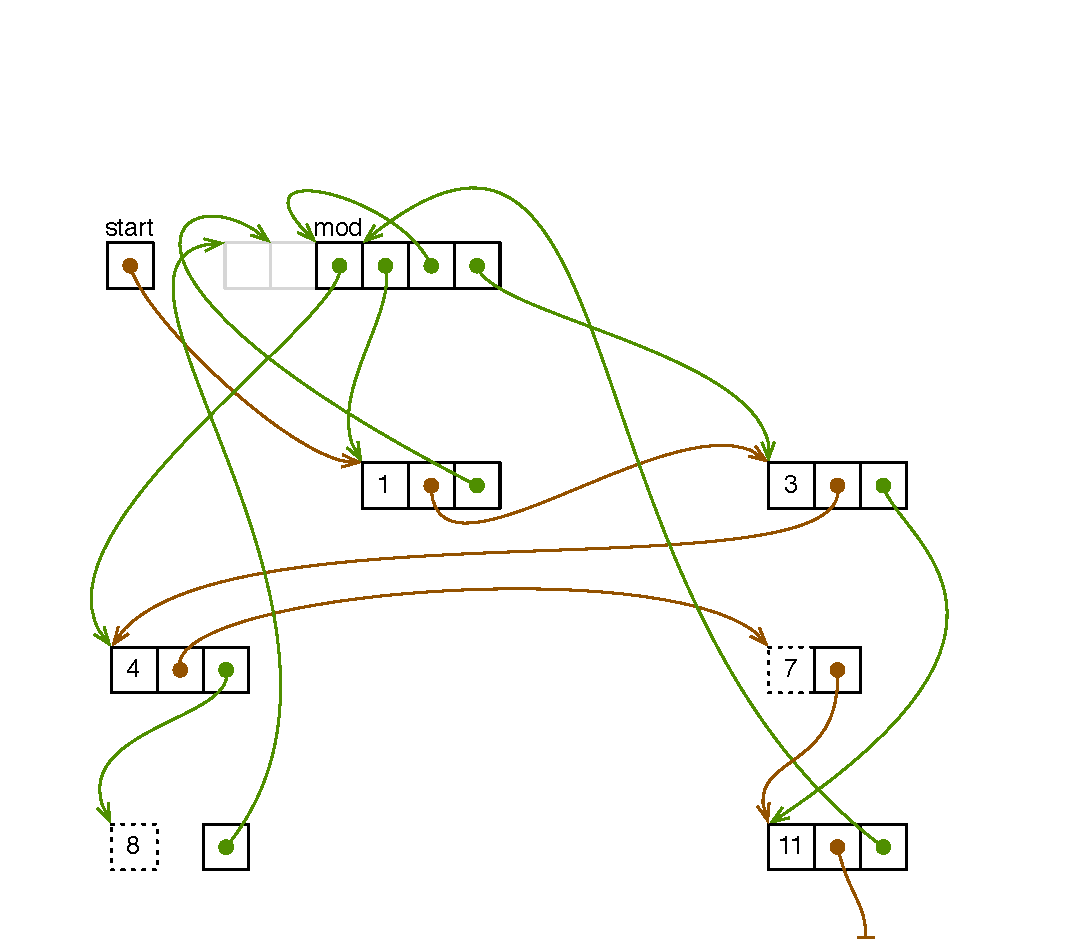
\includegraphics[width=75mm]{undesirablestate.pdf}
\caption{An undesirable state}
\label{fig:undesirablestate}
\end{figure}

\section{Enforcing consistency using boxed assertions}

To enforce the consistency, I propose using the `boxed assertions' concept from RGSep. Rather than splitting the {\tt val} field into two half-permissions, let us form a shared region that comprises all of the {\tt val} fields. If the $list$ and $class$ predicates form two non-unifiable views of the {\tt val} fields, then when they come to be composed, a contradiction will ensue. For instance, if $x_n$ is the address of the node with value $n$ (assuming that all values are distinct) then, in our undesirable state of Fig.~\ref{fig:undesirablestate}, the $list$ predicate would describe the shared region as 
\[
\boxed{x_1.{\tt val}↦1 * x_3.{\tt val}↦3 * x_4.{\tt val}↦4 * x_7.{\tt val}↦7 * x_{11}.{\tt val}↦11}
\]
while the family of $class_i$ predicates would see it as 
\[
\boxed{x_4.{\tt val}↦4 * x_8.{\tt val}↦8 * x_1.{\tt val}↦1 * x_3.{\tt val}↦3 * x_{11}.{\tt val}↦11}.
\]
The $*$-ing together of these two assertions, say $\boxed{P_{list}}$ and $\boxed{P_{class}}$, is equivalent to $\boxed{P_{list} ∧ P_{class}}$, which is simply $\boxed{\false}$.

Let us introduce a new `$\doublestar$' operator to the assertion language. Its main property is that $\boxed{P} \doublestar \boxed{Q}$ is equivalent to $\boxed{P*Q}$. Thus, its semantics shall be defined as follows:
\[
l,s,i⊧p_0\doublestar p_1 ≝ ∃l_0,l_1,s_0,s_1. l{=}l_0⊙ l_1 ∧ s{=}s_0⊙ s_1 ∧ l_0,s_0,i⊧p_0 ∧ l_1,s_1,i⊧p_1
\]
We can now define the state as follows:
\[
state ≝ \begin{array}[t]{@{}l}{\tt start}↦x * {\tt mod}↦c_0,c_1,c_2,c_3 {}\\{} * list(x) * (class_0(c_0) \doublestar class_1(c_1) \doublestar class_2(c_2) \doublestar class_3(c_3)) \end{array}
\]
The double-stars on the second line build up the shared state of the family of $class$ predicates. The single star between that and the $list$ predicate enforces a consistent view of the same shared state. The $list$ and $class$ predicates can be defined like so.
\[
\begin{array}{rcl}
list_n(x) &⇔& x\dot= 0 ∨ ∃x'. x\dot{≠}0 * x.{\tt next}↦x' * (\boxed{x.{\tt val}↦v ∧ v≥n} \doublestar list_v(x')) \\
list(x) &≝& list_0(x) \\
class_n(c) &⇔& c\dot= 0 ∨ ∃c'. c\dot{≠}0 * c.{\tt fd}↦c' * (\boxed{c.{\tt val}↦v ∧ v\text{ mod }4 = n} \doublestar list_n(c',c)) \\
list_n(c,c') &⇔& c\dot= c' ∨ ∃c''. c\dot{≠}c' * c.{\tt fd}↦c'' * (\boxed{c.{\tt val}↦v ∧ v\text{ mod }4 = n} \doublestar list_n(c'',c')) \\
\end{array}
\]

However, the consistency is only being enforced at the topmost level. Thus, I don't think we get the required compositionality that we would like in order to be able to reason locally. For instance, how might we reason about the following program that updates a node in the structure?

\section{A program}

The program changes the value of node {\tt c} to {\tt w}, updating its position in the datastructure accordingly.
\begin{lstlisting}
void setNode(node* c, int w) {
  
  // set c's new value, caching the old one
  int v = c->val;
  c->val = w;
  
  // remove c from list 
  node* p = (node*) (&start - 1);
  while (p->next != c) p = p->next;
  p->next = c->next;
  
  // return c to list
  p = (node*) (&start - 1);
  while ((p->next != 0) && (p->next)->val < w) p = p->next;
  c->next = p->next;
  p->next = c;
  
  // remove c from its old class
  p = (node*) (mod + (v%4) - 2);
  while (p->fd != c) p = p->fd;
  p->fd = c->fd;
  
  // add c to its new class
  p = (node*) (mod + (w%4) - 2);
  c->fd = p->fd;
  p->fd = c;
}
\end{lstlisting}

\section{Mutually-referring boxed regions}

Another approach that might work is to use several different boxes. For this example, we shall have 5 boxes: Boxes 0-3 for each of the classes, and Box 4 for the linked list. Box 4 shall describe a state such as that on the left of Fig.~\ref{fig:twoparts}: the {\tt next} pointers plus half-permission on the {\tt val} fields. Boxes 0-3 shall each describe one of the four separate sections on the right of Fig.~\ref{fig:twoparts}: the {\tt fd} pointers plus the other half-permission on the {\tt val} fields.

Every part of the state thus lies within one of these shared regions: indeed, since they are mutually disjoint, every part of the state lies in \emph{exactly} one of these regions. So we can describe the entire state by $*$-conjoining the five predicates together:
\[
state ≝ \boxed[0]{class_0} * \boxed[1]{class_1} * \boxed[2]{class_2} * \boxed[3]{class_3} * \boxed[4]{list}
\]

We define the $list$ and $class_i$ predicates like so:

\[
\begin{array}{rcl}
lel(x, y) &⇔& \begin{array}[t]{@{}l} ∃m,n. x.{\tt val}\pto[.25]m {}\\{}
* x.{\tt next}↦y * (y\dot=0 ∨ y\dot{≠}0 * y.{\tt val}\pto[.25]n * m\dot{≤}n) \end{array} \\
Lel(x, y) &⇔& \begin{array}[t]{@{}l}∃m,n,i. x.{\tt val}\pto[.25]m {}\\{}
* x.{\tt next}↦y * (y\dot=0 ∨ y\dot{≠}0 * y.{\tt val}\pto[.25]n * m\dot{≤}n) {}\\{}
* i\dot=m\%4 * \boxed[i]{inclass_i(x)}\end{array} \\
cel_i(x,y) &⇔& ∃n. x.{\tt val}\pto[.5]n * n\%4\dot=i * x.{\tt fd}↦y\\
Cel_i(x,y) &⇔& \begin{array}[t]{@{}l} ∃n. x.{\tt val}\pto[.5]n * n\%4\dot=i * x.{\tt fd}↦y {}\\{}
* \boxed[4]{inlist(x)} \end{array}\\
inlist(y) &⇔& ∃x,z. \amp{\tt start}↦x * x.{\tt val}\pto[.25]\_ * lel^*(x, y) * lel^+(y, 0) \\
inclass_i(x) &⇔& ∃y. {\tt mod}{+}i↦y * cel_i^*(y,x) * cel_i^+(x,{\tt mod}{+}i{-}2) \\
list &⇔& ∃y. \amp{\tt start}↦y * (y\dot=0 ∨ y\dot{≠}0 * y.{\tt val}\pto[.25]\_) * Lel^*(y, 0) \\
class_i &⇔& ∃y. {\tt mod}{+}i↦y * Cel_i^*(y,{\tt mod}{+}i{-}2)
\end{array}
\]
Note the following points:
\begin{itemize}
\item `Lel' abbreviates `list element' and `cel' abbreviates `class element'.
\item If $R$ is a binary predicate, then $R^*$ denotes its reflexive transitive closure, defined as the least relation satisfying:
\[
R^*(x,y) \ ⇔\ x\dot=y ∨ ∃x'. x\dot{≠}y * R(x,x') * R^*(x',y)
\]
Then $R^+(x,y)$ means $∃x'. x\dot{≠}y * R(x,x') * R^*(x',y)$.
\item Those predicates that are capitalised carry cross references to other boxed regions. For instance, $Lel(x,y)$ is the same as $lel(x,y)$, except that it additionally states that $x$ appears in its respective equivalence class. Note that $inclass_i(x)$ uses the non-capitalised predicates, so as to avoid circular cross-references.
\item We use quarter-permission pointers in the $lel$ and $Lel$ predicates. The $list$ predicate has a total of half-permission on the {\tt val} fields. The $lel$ and $Lel$ predicates further split this permission in half, because they need to access each {\tt val} field twice: once to compare it to the previous node's {\tt val}, and once to compare it to the next node's {\tt val}. As a result of this, we need to make up the missing quarter-permission on the very first {\tt val}, and this is done in the definitions of $list$ and $inlist$.
\end{itemize}

\section{Verifying the program}

Lemma: $R^*(x,y) \ ⇔\ x\dot=y ∨ ∃y'. x\dot{≠}y * R^*(x,y') * R(y',y)$

\begin{lstlisting}
£\ass{\boxed[0]{class_0} * \boxed[1]{class_1} * \boxed[2]{class_2} * \boxed[3]{class_3} * \boxed[4]{list} * ∃i\in[0,4). \boxed[i]{inclass_i({\tt c})} * \boxed[4]{inlist({\tt c})}}£
// Note the slight weakness in the statement: c must
// be in some class, but not necessarily the right
// one. (Actually, it must be in the right one, because
// we have additionally the class0, class1, class2 and
// class3 predicates that enforce the well-formedness
// of the classes. Perhaps the above definitions should
// be 'weakened' in a similar way?)
void setNode(node* c, int w) {
  £\ass{\boxed[0]{class_0} * \boxed[1]{class_1} * \boxed[2]{class_2} * \boxed[3]{class_3} * \boxed[4]{list} * ∃i\in[0,4). \boxed[i]{inclass_i({\tt c})} {}\\{}
  * \boxed[4]{∃s,n. \amp{\tt start}↦s * s.{\tt val}\pto[.25]\_ * lel^*(s, {\tt c}) * lel({\tt c}, n) * lel^*(n,0)}}£
  £\ass{\boxed[0]{class_0} * \boxed[1]{class_1} * \boxed[2]{class_2} * \boxed[3]{class_3} * \boxed[4]{list} * ∃i\in[0,4). \boxed[i]{inclass_i({\tt c})} {}\\{}
  * \boxed[4]{∃s,n,v,v'. \amp{\tt start}↦s * s.{\tt val}\pto[.25]\_ * lel^*(s, {\tt c}) * {\tt c}.{\tt val}\pto[.25]v {}\\{}
  * {\tt c}.{\tt next}↦n * (n\dot=0 ∨ n\dot{≠}0 * n.{\tt val}\pto[.25]v' * v\dot{≤}v') * lel^*(n,0)}}£
  // Use Lemma from above. 
  £\ass{\boxed[0]{class_0} * \boxed[1]{class_1} * \boxed[2]{class_2} * \boxed[3]{class_3} * \boxed[4]{list} * ∃i\in[0,4). \boxed[i]{inclass_i({\tt c})} {}\\{}
  * \boxed[4]{∃s,p,n,v,v'. \amp{\tt start}↦s * s.{\tt val}\pto[.25]\_ {}\\{}
  * (s\dot={\tt c} ∨ s\dot{≠}{\tt c} * lel^*(s,p) * lel(p,{\tt c})) {}\\{}
  * {\tt c}.{\tt val}\pto[.25]v * {\tt c}.{\tt next}↦n {}\\{}
  * (n\dot=0 ∨ n\dot{≠}0 * n.{\tt val}\pto[.25]v' * v\dot{≤}v') * lel^*(n,0)}}£
  £\ass{\boxed[0]{class_0} * \boxed[1]{class_1} * \boxed[2]{class_2} * \boxed[3]{class_3} * \boxed[4]{list} * ∃i\in[0,4). \boxed[i]{inclass_i({\tt c})} {}\\{}
  * (\boxed[4]{∃n,v,v'. \amp{\tt start}↦ {\tt c} * {\tt c}.{\tt val}\pto[.5]v * {\tt c}.{\tt next}↦n {}\\{}
  * (n\dot=0 ∨ n\dot{≠}0 * n.{\tt val}\pto[.25]v' * v\dot{≤}v') * lel^*(n,0)}
  ∨ \boxed[4]{∃s,p,n,v,v'. \amp{\tt start}↦s * s.{\tt val}\pto[.25]\_ {}\\{}
  * s\dot{≠}{\tt c} * lel^*(s,p) * lel(p,{\tt c}) {}\\{}
  * {\tt c}.{\tt val}\pto[.25]v * {\tt c}.{\tt next}↦n {}\\{}
  * (n\dot=0 ∨ n\dot{≠}0 * n.{\tt val}\pto[.25]v' * v\dot{≤}v') * lel^*(n,0)})}£
  £\ass{\boxed[0]{class_0} * \boxed[1]{class_1} * \boxed[2]{class_2} * \boxed[3]{class_3} * \boxed[4]{list} * ∃i\in[0,4). \boxed[i]{inclass_i({\tt c})} {}\\{}
  * (\boxed[4]{∃n,v,v'. \amp{\tt start}↦ {\tt c} * {\tt c}.{\tt val}\pto[.5]v * {\tt c}.{\tt next}↦n {}\\{}
  * (n\dot=0 ∨ n\dot{≠}0 * n.{\tt val}\pto[.25]v' * v\dot{≤}v') * lel^*(n,0)}
  ∨ \boxed[4]{∃s,p,n,u,v,v'',v'. \amp{\tt start}↦s * s.{\tt val}\pto[.25]\_ {}\\{}
  * s\dot{≠}{\tt c} * lel^*(s,p) * p.{\tt val}\pto[.25]u * p.{\tt next}↦{\tt c} {}\\{}
  * ({\tt c}\dot=0 ∨ {\tt c}\dot{≠}0 * {\tt c}.{\tt val}\pto[.25]v'' * u\dot{≤}v'') {}\\{}
  * {\tt c}.{\tt val}\pto[.25]v * {\tt c}.{\tt next}↦n {}\\{}
  * (n\dot=0 ∨ n\dot{≠}0 * n.{\tt val}\pto[.25]v' * v\dot{≤}v') * lel^*(n,0)})}£
  £\ass{\boxed[0]{class_0} * \boxed[1]{class_1} * \boxed[2]{class_2} * \boxed[3]{class_3} * \boxed[4]{list} * ∃i\in[0,4). \boxed[i]{inclass_i({\tt c})} {}\\{}
  * (\boxed[4]{∃n,v,v'. \amp{\tt start}↦ {\tt c} * {\tt c}.{\tt val}\pto[.5]v * {\tt c}.{\tt next}↦n {}\\{}
  * (n\dot=0 ∨ n\dot{≠}0 * n.{\tt val}\pto[.25]v' * v\dot{≤}v') * lel^*(n,0)}
  ∨ \boxed[4]{∃s,p,n,u,v,v'. \amp{\tt start}↦s * s.{\tt val}\pto[.25]\_ {}\\{}
  * s\dot{≠}{\tt c} * lel^*(s,p) * p.{\tt val}\pto[.25]u * p.{\tt next}↦{\tt c} {}\\{}
  * {\tt c}.{\tt val}\pto[.5]v * u\dot{≤}v * {\tt c}.{\tt next}↦n {}\\{}
  * (n\dot=0 ∨ n\dot{≠}0 * n.{\tt val}\pto[.25]v' * v\dot{≤}v') * lel^*(n,0)})}£
  £\ass{\boxed[0]{class_0} * \boxed[1]{class_1} * \boxed[2]{class_2} * \boxed[3]{class_3} * \boxed[4]{list} * ∃i\in[0,4). \boxed[i]{inclass_i({\tt c})} {}\\{}
  * (\boxed[4]{∃p,n,u,v,v'. (\amp{\tt start}↦ {\tt c} {}\\{}
  ∨ \amp{\tt start}↦s * s\dot{≠}{\tt c} * s.{\tt val}\pto[.25]\_ * lel^*(s,p) * p.{\tt val}\pto[.25]u * u\dot{≤}v * p.{\tt next}↦{\tt c}) {}\\{}
  * {\tt c}.{\tt val}\pto[.5]v * {\tt c}.{\tt next}↦n * (n\dot=0 ∨ n\dot{≠}0 * n.{\tt val}\pto[.25]v' * v\dot{≤}v') * lel^*(n,0)})}£
  // We've now accumulated half permission on c.val in both disjuncts. 
  // Now we need the other half from one of the classes.
  £\ass{∃v,i. i\dot=v\%4 * \boxed[0]{class_0} * \boxed[1]{class_1} * \boxed[2]{class_2} * \boxed[3]{class_3} * \boxed[4]{list} {}\\{}
  * (\boxed[4]{∃p,n,u,v'. (\amp{\tt start}↦ {\tt c} {}\\{}
  ∨ \amp{\tt start}↦s * s\dot{≠}{\tt c} * s.{\tt val}\pto[.25]\_ * lel^*(s,p) * p.{\tt val}\pto[.25]u * u\dot{≤}v * p.{\tt next}↦{\tt c}) {}\\{}
  * {\tt c}.{\tt val}\pto[.5]v * {\tt c}.{\tt next}↦n * (n\dot=0 ∨ n\dot{≠}0 * n.{\tt val}\pto[.25]v' * v\dot{≤}v') * lel^*(n,0)}) {}\\{}
  * \boxed[i]{inclass_i({\tt c})}}£
  £\ass{∃v,i. i\dot=v\%4 * \boxed[0]{class_0} * \boxed[1]{class_1} * \boxed[2]{class_2} * \boxed[3]{class_3} * \boxed[4]{list} {}\\{}
  * (\boxed[4]{∃p,n,u,v'. (\amp{\tt start}↦ {\tt c} {}\\{}
  ∨ \amp{\tt start}↦s * s\dot{≠}{\tt c} * s.{\tt val}\pto[.25]\_ * lel^*(s,p) * p.{\tt val}\pto[.25]u * u\dot{≤}v * p.{\tt next}↦{\tt c}) {}\\{}
  * {\tt c}.{\tt val}\pto[.5]v * {\tt c}.{\tt next}↦n * (n\dot=0 ∨ n\dot{≠}0 * n.{\tt val}\pto[.25]v' * v\dot{≤}v') * lel^*(n,0)}) {}\\{}
  * \boxed[i]{ ∃m. {\tt mod}{+}i↦m * cel_i^*(m,{\tt c}) * cel_i^+({\tt c},{\tt mod}{+}i{-}2)}}£
  £\ass{∃v,i. i\dot=v\%4 * \boxed[0]{class_0} * \boxed[1]{class_1} * \boxed[2]{class_2} * \boxed[3]{class_3} * \boxed[4]{list} {}\\{}
  * (\boxed[4]{∃p,n,u,v'. (\amp{\tt start}↦ {\tt c} {}\\{}
  ∨ \amp{\tt start}↦s * s\dot{≠}{\tt c} * s.{\tt val}\pto[.25]\_ * lel^*(s,p) * p.{\tt val}\pto[.25]u * u\dot{≤}v * p.{\tt next}↦{\tt c}) {}\\{}
  * {\tt c}.{\tt val}\pto[.5]v * {\tt c}.{\tt next}↦n * (n\dot=0 ∨ n\dot{≠}0 * n.{\tt val}\pto[.25]v' * v\dot{≤}v') * lel^*(n,0)}) {}\\{}
  * \boxed[i]{∃m,f. {\tt mod}{+}i↦m * cel_i^*(m,{\tt c}) * cel_i({\tt c},f) * cel_i^*(f,{\tt mod}{+}i{-}2)}}£
  £\ass{∃v,i. i\dot=v\%4 * \boxed[0]{class_0} * \boxed[1]{class_1} * \boxed[2]{class_2} * \boxed[3]{class_3} * \boxed[4]{list} {}\\{}
  * (\boxed[4]{∃p,n,u,v'. (\amp{\tt start}↦ {\tt c} {}\\{}
  ∨ \amp{\tt start}↦s * s\dot{≠}{\tt c} * s.{\tt val}\pto[.25]\_ * lel^*(s,p) * p.{\tt val}\pto[.25]u * u\dot{≤}v * p.{\tt next}↦{\tt c}) {}\\{}
  * {\tt c}.{\tt val}\pto[.5]v * {\tt c}.{\tt next}↦n * (n\dot=0 ∨ n\dot{≠}0 * n.{\tt val}\pto[.25]v' * v\dot{≤}v') * lel^*(n,0)}) {}\\{}
  * \boxed[i]{∃m,f. {\tt mod}{+}i↦m * cel_i^*(m,{\tt c}) * {\tt c}.{\tt val}\pto[.5]v * {\tt c}.{\tt fd}↦f * cel_i^*(f,{\tt mod}{+}i{-}2)}}£
  // We now have complete ownership of c.val (although
  // it is spread across two different boxed regions

  // set c's new value, caching the old one
  int v = c->val;
  £\ass{∃i. i\dot={\tt v}\%4 * \boxed[0]{class_0} * \boxed[1]{class_1} * \boxed[2]{class_2} * \boxed[3]{class_3} * \boxed[4]{list} {}\\{}
  * (\boxed[4]{∃p,n,u,v'. (\amp{\tt start}↦ {\tt c} {}\\{}
  ∨ \amp{\tt start}↦s * s\dot{≠}{\tt c} * s.{\tt val}\pto[.25]\_ * lel^*(s,p) * p.{\tt val}\pto[.25]u * u\dot{≤}{\tt v} * p.{\tt next}↦{\tt c}) {}\\{}
  * {\tt c}.{\tt val}\pto[.5]{\tt v} * {\tt c}.{\tt next}↦n * (n\dot=0 ∨ n\dot{≠}0 * n.{\tt val}\pto[.25]v' * {\tt v}\dot{≤}v') * lel^*(n,0)}) {}\\{}
  * \boxed[i]{∃m,f. {\tt mod}{+}i↦m * cel_i^*(m,{\tt c}) * {\tt c}.{\tt val}\pto[.5]{\tt v} * {\tt c}.{\tt fd}↦f * cel_i^*(f,{\tt mod}{+}i{-}2)}}£
  c->val = w;
  £\ass{∃i. i\dot={\tt v}\%4 * \boxed[0]{class_0} * \boxed[1]{class_1} * \boxed[2]{class_2} * \boxed[3]{class_3} * \boxed[4]{list} {}\\{}
  * (\boxed[4]{∃p,n,u,v'. (\amp{\tt start}↦ {\tt c} {}\\{}
  ∨ \amp{\tt start}↦s * s\dot{≠}{\tt c} * s.{\tt val}\pto[.25]\_ * lel^*(s,p) * p.{\tt val}\pto[.25]u * u\dot{≤}{\tt v} * p.{\tt next}↦{\tt c}) {}\\{}
  * {\tt c}.{\tt val}\pto[.5]{\tt w} * {\tt c}.{\tt next}↦n * (n\dot=0 ∨ n\dot{≠}0 * n.{\tt val}\pto[.25]v' * {\tt v}\dot{≤}v') * lel^*(n,0)}) {}\\{}
  * \boxed[i]{∃m,f. {\tt mod}{+}i↦m * cel_i^*(m,{\tt c}) * {\tt c}.{\tt val}\pto[.5]{\tt w} * {\tt c}.{\tt fd}↦f * cel_i^*(f,{\tt mod}{+}i{-}2)}}£
  // But now we have a contradiction, because we have 
  // two differing views of boxed region 4.
  
  // remove c from list 
  node* p = (node*) (&start - 1);
  while (p->next != c) p = p->next;
  p->next = c->next;
  
  // return c to list
  p = (node*) (&start - 1);
  while ((p->next != 0) && (p->next)->val < w) p = p->next;
  c->next = p->next;
  p->next = c;
  
  // remove c from its old class
  p = (node*) (mod + (v%4) - 2);
  while (p->fd != c) p = p->fd;
  p->fd = c->fd;
  
  // add c to its new class
  p = (node*) (mod + (w%4) - 2);
  c->fd = p->fd;
  p->fd = c;
}
\end{lstlisting}

Let us now expand out an instance of these predicates, to see how the double-star and the single star interact. We will demonstrate a possible state that comprises nodes with values 2,4,7 and 9. \footnotesize
\[
\begin{array}{rcl}
l,s ⊧ state &⇔& 
\begin{array}[t]{@{}l}
l = \{start ↦ x, mod↦(c_0,c_1,c_2,c_3)\}+l_i+l_c {}\\{}
    ∧ l_i,s ⊧ list(x) {}\\{}
    ∧ l_c,s ⊧ class_0(c_0) \doublestar class_1(c_1) \doublestar class_2(c_2) \doublestar class_3(c_3)
\end{array} \\
&⇔& 
\begin{array}[t]{@{}l}
l = \{start ↦ x, mod↦(c_0,c_1,c_2,c_3)\}+l_i+l_0+l_1+l_2+l_3 {}\\{}
    ∧ l_i,s ⊧ list(x) {}\\{}
    ∧ s = s_0+s_1+s_2+s_3 {}\\{}
    ∧ l_0,s_0 ⊧ class_0(c_0) ∧ l_1,s_1 ⊧ class_1(c_1) {}\\{}
    ∧ l_2,s_2 ⊧ class_2(c_2) ∧ l_3,s_3 ⊧ class_3(c_3)
\end{array} \\ \hline
l_0,s_0 ⊧ class_0(c_0) &⇔& 
\begin{array}[t]{@{}l}
l_0 = \{c_0.{\tt fd}↦c_0'\} + l_0' {}\\{}
∧ l_0',s_0 ⊧ \boxed{c_0.{\tt val}↦v ∧ v\text{ mod }4 = 0} \doublestar list_n(c_0',c_0)
\end{array} \\
&⇐& 
\begin{array}[t]{@{}l}
l_0 = \{c_0.{\tt fd}↦c_0'\} + l_0' {}\\{}
∧ s_0 = \{c_0.{\tt val}↦4\} + s_0' {}\\{}
∧ l_0',s_0' ⊧ list_n(c_0',c_0)
\end{array} \\
&⇐& 
\begin{array}[t]{@{}l}
l_0 = \{c_0.{\tt fd}↦c_0'\} + l_0' {}\\{}
∧ s_0 = \{c_0.{\tt val}↦4\} + s_0' {}\\{}
∧ l_0',s_0' ⊧ c_0'\dot=c_0
\end{array} \\
&⇔& l_0 = \{c_0.{\tt fd}↦c_0\} ∧ s_0 = \{c_0.{\tt val}↦4\} \\ \hline
l,s ⊧ state &⇐& 
\begin{array}[t]{@{}l}
l = \{start ↦ x, mod↦(c_0,c_1,c_2,c_3)\}+l_i+l_0+l_1+l_2+l_3 {}\\{}
    ∧ l_i,s ⊧ list(x) {}\\{}
    ∧ s = s_0+s_1+s_2+s_3 {}\\{}
    ∧ l_0 = \{c_0.{\tt fd}↦c_0\} ∧ s_0 = \{c_0.{\tt val}↦4\} {}\\{}
    ∧ l_1 = \{c_1.{\tt fd}↦c_1\} ∧ s_1 = \{c_1.{\tt val}↦9\} {}\\{}
    ∧ l_2 = \{c_2.{\tt fd}↦c_2\} ∧ s_2 = \{c_2.{\tt val}↦2\} {}\\{}
    ∧ l_3 = \{c_3.{\tt fd}↦c_3\} ∧ s_3 = \{c_3.{\tt val}↦7\}
\end{array} \\
&⇔& 
\begin{array}[t]{@{}l}
l = \{start ↦ x, mod↦(c_0,c_1,c_2,c_3), c_0.{\tt fd}↦c_0, c_1.{\tt fd}↦c_1, c_2.{\tt fd}↦c_2, c_3.{\tt fd}↦c_3\}+l_i {}\\{}
    ∧ s = \{c_0.{\tt val}↦4, c_1.{\tt val}↦9, c_2.{\tt val}↦2, c_3.{\tt val}↦7\} {}\\{}
    ∧ l_i,s ⊧ list(x)
\end{array} \\ \hline
l_i,s ⊧ list_0(x) &⇔&
\begin{array}[t]{@{}l}
l_i = \{x.{\tt next}↦x'\} + l_i' {}\\{}
∧ l_i',s ⊧ \boxed{x.{\tt val}↦v ∧ v≥n} \doublestar list_v(x')
\end{array} \\
&⇐&
\begin{array}[t]{@{}l}
l_i = \{x.{\tt next}↦x'\} + l_i' {}\\{}
∧ s= \{x.{\tt val}↦2\}+s' {}\\{}
∧ l_i',s' ⊧ list_2(x')
\end{array} \\
&⇐&
\begin{array}[t]{@{}l}
l_i = \{x.{\tt next}↦x', x'.{\tt next}↦x''\} + l_i'' {}\\{}
∧ s= \{x.{\tt val}↦2, x'.{\tt val}↦4\}+s'' {}\\{}
∧ l_i'',s'' ⊧ list_4(x'')
\end{array} \\
&⇐&
\begin{array}[t]{@{}l}
l_i = \{x.{\tt next}↦x', x'.{\tt next}↦x'', x''.{\tt next}↦x'''\} + l_i''' {}\\{}
∧ s= \{x.{\tt val}↦2, x'.{\tt val}↦4, x''.{\tt val}↦7\}+s''' {}\\{}
∧ l_i''',s''' ⊧ list_7(x''')
\end{array} \\
&⇐&
\begin{array}[t]{@{}l}
l_i = \{x.{\tt next}↦x', x'.{\tt next}↦x'', x''.{\tt next}↦x''', x'''.{\tt next}↦x''''\} + l_i'''' {}\\{}
∧ s= \{x.{\tt val}↦2, x'.{\tt val}↦4, x''.{\tt val}↦7, x'''.{\tt val}↦9\}+s'''' {}\\{}
∧ l_i'''',s'''' ⊧ list_9(x'''')
\end{array} \\
&⇐&
\begin{array}[t]{@{}l}
l_i = \{x.{\tt next}↦x', x'.{\tt next}↦x'', x''.{\tt next}↦x''', x'''.{\tt next}↦\bot\}{}\\{}
∧ s= \{x.{\tt val}↦2, x'.{\tt val}↦4, x''.{\tt val}↦7, x'''.{\tt val}↦9\}
\end{array} \\ \hline
l,s ⊧ state &⇐& 
\begin{array}[t]{@{}l}
l = \{start ↦ x, mod↦(c_0,c_1,c_2,c_3), c_0.{\tt fd}↦c_0, c_1.{\tt fd}↦c_1, c_2.{\tt fd}↦c_2, c_3.{\tt fd}↦c_3\}+l_i {}\\{}
    ∧ s = \{c_0.{\tt val}↦4, c_1.{\tt val}↦9, c_2.{\tt val}↦2, c_3.{\tt val}↦7\} {}\\{}
    ∧ l_i = \{x.{\tt next}↦x', x'.{\tt next}↦x'', x''.{\tt next}↦x''', x'''.{\tt next}↦\bot\}{}\\{}
    ∧ s= \{x.{\tt val}↦2, x'.{\tt val}↦4, x''.{\tt val}↦7, x'''.{\tt val}↦9\}
\end{array} \\
&⇔& 
\begin{array}[t]{@{}l}
l = \{start ↦ c_2, mod↦(c_0,c_1,c_2,c_3), {}\\{}
    c_0.{\tt fd}↦c_0, c_1.{\tt fd}↦c_1, c_2.{\tt fd}↦c_2, c_3.{\tt fd}↦c_3, {}\\{}
    c_2.{\tt next}↦c_0, c_0.{\tt next}↦c_3, c_3.{\tt next}↦c_1, c_1.{\tt next}↦\bot\} {}\\{}
    ∧ s = \{c_0.{\tt val}↦4, c_1.{\tt val}↦9, c_2.{\tt val}↦2, c_3.{\tt val}↦7\}
\end{array} \\
\end{array} 
\]


\end{document}